\documentclass[a4paper,12pt]{article}

\usepackage[utf8]{inputenc}
\usepackage[T2A]{fontenc}
\usepackage[russian]{babel}
\usepackage{amsmath,amssymb}
\usepackage{graphicx}
\usepackage{booktabs}
\usepackage{geometry}
\usepackage{hyperref}
\usepackage{float}

\geometry{margin=2cm}

\title{Проект по оптимальному инвестированию\\[0.3em]
\large Модель связи валютного курса EUR/USD и цены на нефть Brent}
\author{}
\date{10 марта 2026 года}

\begin{document}

\maketitle

\section*{1. Обзор литературы и постановка задачи}
В качестве отправной точки я взял три статьи, которые были даны для проекта.

\textbf{1) Benlaria, Gheraia, Belbali et al. (2020).}
Авторы исследуют месячные данные за январь 1999 --- октябрь 2019 и оценивают связь между ценой нефти, курсом EUR/USD и ценой золота с помощью модели ARDL. Их основной вывод состоит в том, что между переменными есть связь, но она проявляется в первую очередь в краткосрочной динамике; дополнительно тест Грейнджера указывает на однонаправленную причинность от EUR/USD к нефти.

\textbf{2) Fratzscher, Schneider, Van Robays (2014).}
В рабочей статье ЕЦБ связь нефти, доллара США и других финансовых активов рассматривается с точки зрения финансового рынка. Авторы подчеркивают, что с начала 2000-х связь между нефтью и долларом стала заметно теснее, а причинность стала двусторонней. Важный для меня вывод из этой статьи состоит в том, что знак и сила связи могут меняться по режимам рынка.

\textbf{3) Dias, Galv\~ao, Alexandre et al. (2025).}
Авторы изучают более свежий период, с 3 января 2022 года по 8 декабря 2024 года, и анализируют влияние нефти и нефтяной волатильности на основные валютные пары. Для EUR/USD они подчеркивают, что связь с нефтяным фактором существует, но сама валютная динамика зависит и от поведения других крупных валютных рынков. Это полезно как аргумент в пользу того, что в последние годы чистая связь ``нефть $\to$ EUR/USD'' могла ослабнуть.

Из этих работ естественно вытекает следующая задача: \textit{проверить, существует ли на воспроизводимых данных устойчивая эмпирическая связь между ценой нефти Brent и курсом EUR/USD, и одинаково ли она проявляется в долгом и коротком горизонтах.}

Практический смысл задачи для оптимального инвестирования такой. Если рост нефти систематически связан с ослаблением доллара и ростом EUR/USD, то нефть можно рассматривать как фактор хеджирования валютного риска и как индикатор для ребалансировки позиций в валютных стратегиях.

\section*{2. Данные}
Для эмпирической части я использовал открытые ряды FRED:
\begin{itemize}
    \item \texttt{DEXUSEU} --- курс USD за 1 EUR, то есть ряд EUR/USD в долларовом выражении;
    \item \texttt{DCOILBRENTEU} --- цена нефти Brent в долларах за баррель.
\end{itemize}

Дневная выборка после синхронизации наблюдений покрывает период с 14 января 2000 года по 2 марта 2026 года. Для краткосрочных регрессий я использую подвыборку с 4 января 2010 года, чтобы исключить слишком далекий ранний участок и сделать режимы более сопоставимыми. Для долгосрочного анализа я перехожу к месячным средним и беру период с января 1999 года по февраль 2026 года.

Обозначим
\[
e_t=\ln(\text{EUR/USD}_t), \qquad o_t=\ln(\text{Brent}_t).
\]
Тогда краткосрочные изменения описываются логарифмическими доходностями
\[
\Delta e_t=e_t-e_{t-1}, \qquad \Delta o_t=o_t-o_{t-1}.
\]

Описательная статистика для дневных лог-доходностей приведена в таблице.

\begin{center}
\begin{tabular}{lrrrrr}
\toprule
series & mean & std & min & max & obs \\
\midrule
EUR/USD daily log return & 0.0000 & 0.0058 & -0.0300 & 0.0462 & 6468 \\
Brent daily log return & 0.0002 & 0.0263 & -0.6437 & 0.4120 & 6468 \\
\bottomrule
\end{tabular}

\end{center}

Из таблицы видно, что нефть существенно более волатильна, чем EUR/USD, что соответствует и экономической интуиции, и выводам литературы.

\section*{3. Теоретическая модель}
Я использую две взаимодополняющие спецификации.

\textbf{Краткосрочная модель.}
Для дневных данных оценивается регрессия
\[
\Delta e_t=\alpha+\beta_0 \Delta o_t+\beta_1 \Delta o_{t-1}+\gamma \Delta e_{t-1}+\varepsilon_t.
\]
Экономический смысл коэффициента $\beta_0$ такой: если рост цены нефти обычно сопровождается ослаблением доллара, то курс EUR/USD должен расти, и тогда ожидается $\beta_0>0$.

\textbf{Долгосрочная модель.}
Для месячных данных сначала рассматривается долгосрочное соотношение
\[
e_t=c+\theta o_t+u_t.
\]
Если остаток $u_t$ стационарен, то можно говорить о коинтеграции между курсом и нефтью. Тогда корректно рассматривать модель исправления ошибок
\[
\Delta e_t=\alpha+\delta_0 \Delta o_t+\delta_1 \Delta o_{t-1}
+\rho \Delta e_{t-1}+\lambda u_{t-1}+\varepsilon_t.
\]
Здесь коэффициент $\lambda$ показывает скорость возврата к долгосрочному равновесию. Для содержательной модели обычно ожидается
\[
\lambda<0.
\]
Чем он по модулю больше, тем быстрее курс возвращается к долгосрочной траектории после отклонения.

Кроме того, я использую:
\begin{itemize}
    \item ADF-тесты на стационарность уровней и доходностей;
    \item тест Энгла--Грейнджера на коинтеграцию;
    \item тесты Грейнджера для месячных доходностей;
    \item 252-дневную скользящую корреляцию для визуализации смены режимов.
\end{itemize}

\section*{4. Теоретические результаты}
ADF-тесты дают стандартную картину: уровень EUR/USD нестационарен, тогда как лог-доходности обеих переменных стационарны.

\begin{center}
\begin{tabular}{llrr}
\toprule
series & sample & adf\_stat & p\_value \\
\midrule
log EUR/USD level & 1999-01 to latest complete month & -1.9384 & 0.3142 \\
log Brent level & 1999-01 to latest complete month & -2.8872 & 0.0469 \\
EUR/USD log return & 1999-02 to latest complete month & -11.5380 & 0.0000 \\
Brent log return & 1999-02 to latest complete month & -12.7130 & 0.0000 \\
\bottomrule
\end{tabular}

\end{center}

Это подтверждает, что строить краткосрочную модель в доходностях методологически правильно.

Далее я проверил коинтеграцию на трех горизонтах: до 2022 года, после 2022 года и на всей месячной выборке.

\begin{center}
\begin{tabular}{lrrr}
\toprule
sample & obs & coint\_stat & p\_value \\
\midrule
1999-2021 & 275 & -3.0217 & 0.1051 \\
2022-latest & 50 & -1.9465 & 0.5563 \\
Full monthly sample & 325 & -2.6277 & 0.2266 \\
\bottomrule
\end{tabular}

\end{center}

Здесь получается важный вывод. Для периода 1999--2021 $p$-value теста Энгла--Грейнджера равно примерно $0.105$, то есть связь находится на границе статистической значимости на уровне $10\%$, но не подтверждается на более жестком уровне $5\%$. После 2022 года признаков долгосрочной коинтеграции уже нет. Значит, долгосрочная связь между нефтью и EUR/USD в данных скорее слабая и режимно-зависимая, а не жесткая и постоянная.

Если все же оценить долгосрочное уравнение для периода 1999--2021, получается положительный коэффициент при логарифме цены нефти:

\begin{center}
\begin{tabular}{lrrr}
\toprule
variable & coef & std\_err & p\_value \\
\midrule
const & -0.6107 & 0.0393 & 0.0000 \\
log Brent & 0.1961 & 0.0097 & 0.0000 \\
\bottomrule
\end{tabular}

\end{center}

То есть в среднем более высокая цена нефти ассоциируется с более высоким курсом EUR/USD, что согласуется с гипотезой об ослаблении доллара при росте нефти. Однако сам факт коинтеграции остается лишь пограничным, поэтому этот результат нужно интерпретировать аккуратно.

Модель исправления ошибок для периода 1999--2021 имеет вид:

\begin{center}
\begin{tabular}{lrrr}
\toprule
variable & coef & std\_err & p\_value \\
\midrule
const & -0.0002 & 0.0013 & 0.8949 \\
d\_brent & 0.0363 & 0.0149 & 0.0148 \\
d\_brent\_l1 & 0.0039 & 0.0127 & 0.7587 \\
d\_eurusd\_l1 & 0.2859 & 0.0550 & 0.0000 \\
ecm\_l1 & -0.0300 & 0.0166 & 0.0714 \\
\bottomrule
\end{tabular}

\end{center}

Из нее следуют два вывода.
\begin{itemize}
    \item Коэффициент при текущем изменении нефти положителен и статистически значим: рост нефти в текущем месяце связан с ростом EUR/USD в текущем месяце.
    \item Коэффициент при ошибке коррекции $\lambda \approx -0.03$ имеет правильный отрицательный знак, но его значимость лишь пограничная. Это означает медленное и не слишком устойчиво подтверждаемое возвращение к долгосрочному равновесию.
\end{itemize}

Наконец, тесты Грейнджера на месячных доходностях не дают убедительных оснований утверждать, что нефть устойчиво предсказывает EUR/USD или наоборот:

\begin{center}
\begin{tabular}{rrr}
\toprule
lag & oil\_to\_fx\_p & fx\_to\_oil\_p \\
\midrule
1 & 0.4618 & 0.2591 \\
2 & 0.6118 & 0.2127 \\
3 & 0.6560 & 0.2618 \\
\bottomrule
\end{tabular}

\end{center}

Таким образом, мой теоретический итог по данным такой: \textit{стабильной сильной причинной долгосрочной связи я не нахожу, но в краткосрочной динамике положительный совместный эффект нефти и EUR/USD виден достаточно отчетливо.}

\section*{5. Программная часть}
Вся вычислительная часть вынесена в файл \texttt{src/analysis.py}. Скрипт делает следующее:
\begin{itemize}
    \item скачивает оба временных ряда напрямую из FRED;
    \item сохраняет сырые и объединенные данные в папку \texttt{data/};
    \item строит дневные и месячные преобразования;
    \item оценивает регрессии, коинтеграцию и ECM;
    \item сохраняет таблицы в \texttt{csv} и \texttt{tex};
    \item строит графики в папку \texttt{results/}.
\end{itemize}

Основной дневной регрессионный результат приведен ниже.

\begin{center}
\begin{tabular}{lrrr}
\toprule
variable & coef & std\_err & p\_value \\
\midrule
const & -0.0001 & 0.0001 & 0.5275 \\
r\_brent & 0.0141 & 0.0051 & 0.0057 \\
r\_brent\_l1 & 0.0031 & 0.0031 & 0.3288 \\
r\_eurusd\_l1 & 0.0210 & 0.0168 & 0.2135 \\
\bottomrule
\end{tabular}

\end{center}

Коэффициент при текущей доходности нефти равен примерно $0.014$ и статистически значим. Это означает, что рост нефти на $10\%$ в среднем связан с ростом EUR/USD примерно на $0.14\%$ в тот же день. Сам эффект по величине не очень большой, но он устойчиво положителен.

Чтобы проверить идею из статьи ЕЦБ о смене режимов, я разбил выборку на два периода: до 2022 года и после 2022 года.

\begin{center}
\resizebox{\textwidth}{!}{\begin{tabular}{lrrrrrrrrr}
\toprule
sample & obs & beta\_current\_oil & p\_current\_oil & beta\_lagged\_oil & p\_lagged\_oil & beta\_fx\_lag & p\_fx\_lag & r\_squared & corr\_oil\_fx \\
\midrule
Full sample (2010-01-04 to latest) & 3983.0000 & 0.0141 & 0.0057 & 0.0031 & 0.3288 & 0.0210 & 0.2135 & 0.0058 & 0.0712 \\
Pre-2022 sample & 2966.0000 & 0.0162 & 0.0094 & 0.0012 & 0.7494 & 0.0280 & 0.1427 & 0.0080 & 0.0847 \\
2022+ sample & 1016.0000 & 0.0039 & 0.7088 & 0.0119 & 0.0795 & -0.0037 & 0.9177 & 0.0033 & 0.0202 \\
\bottomrule
\end{tabular}
}
\end{center}

Получается важный прикладной результат:
\begin{itemize}
    \item на выборке до 2022 года эффект нефти положителен и значим;
    \item на выборке 2022+ связь почти исчезает статистически.
\end{itemize}

Это хорошо согласуется с литературой: связь между нефтью и курсом не фиксирована навсегда, а зависит от состояния мирового финансового рынка, геополитики и поведения самого доллара как резервной валюты.

На рисунке ниже показана нормированная динамика уровней.

\begin{figure}[H]
\centering
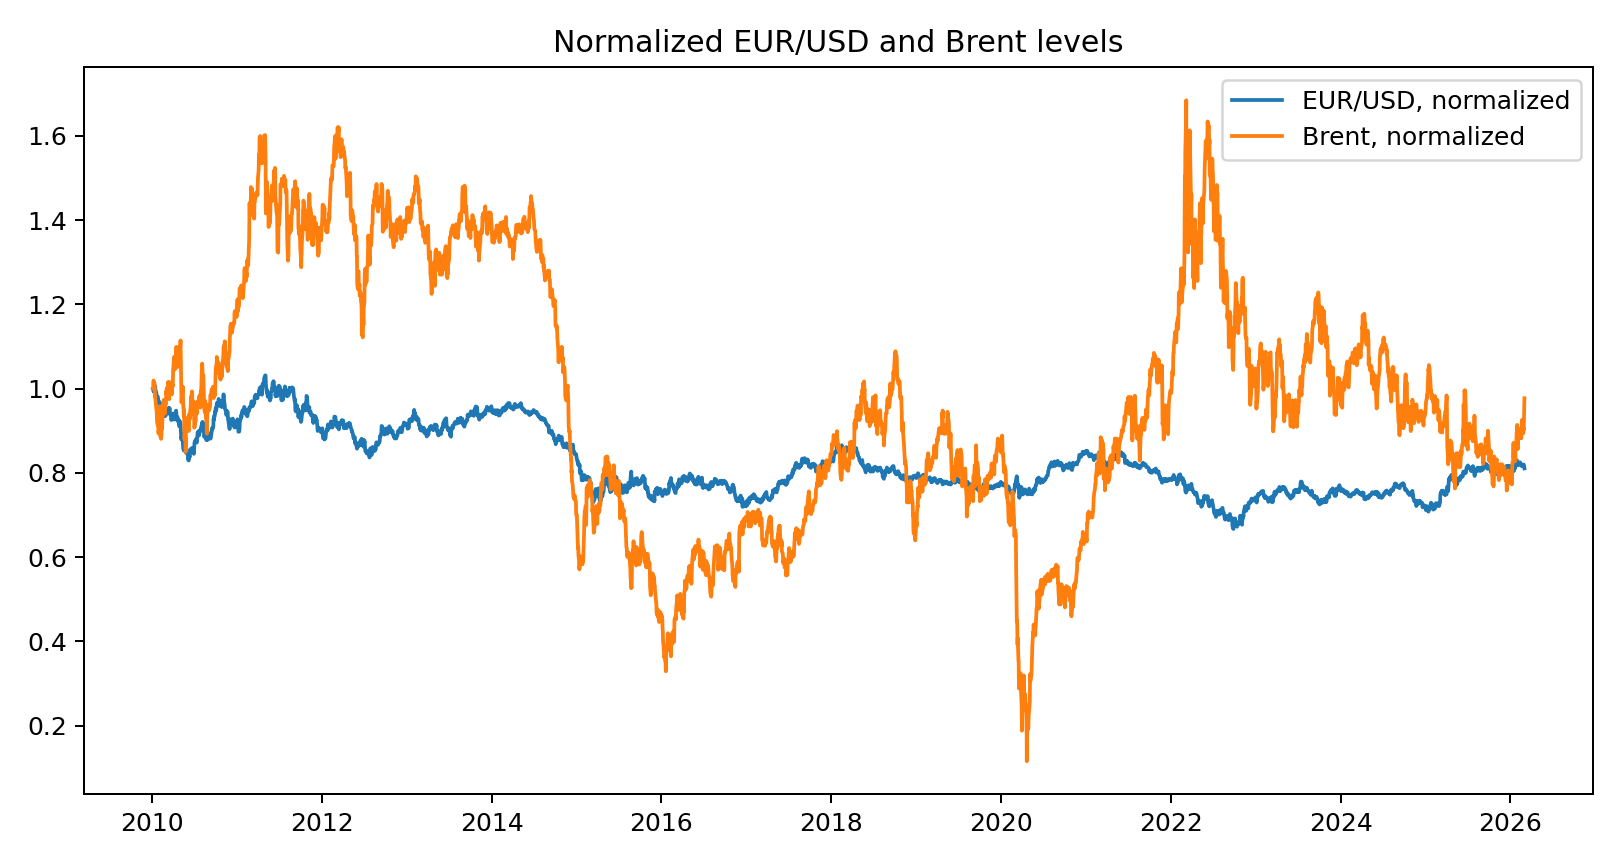
\includegraphics[width=0.88\textwidth]{results/normalized_levels.png}
\caption{Нормированные уровни EUR/USD и Brent}
\end{figure}

Следующий рисунок особенно полезен для интерпретации: он показывает 252-дневную скользящую корреляцию доходностей.

\begin{figure}[H]
\centering
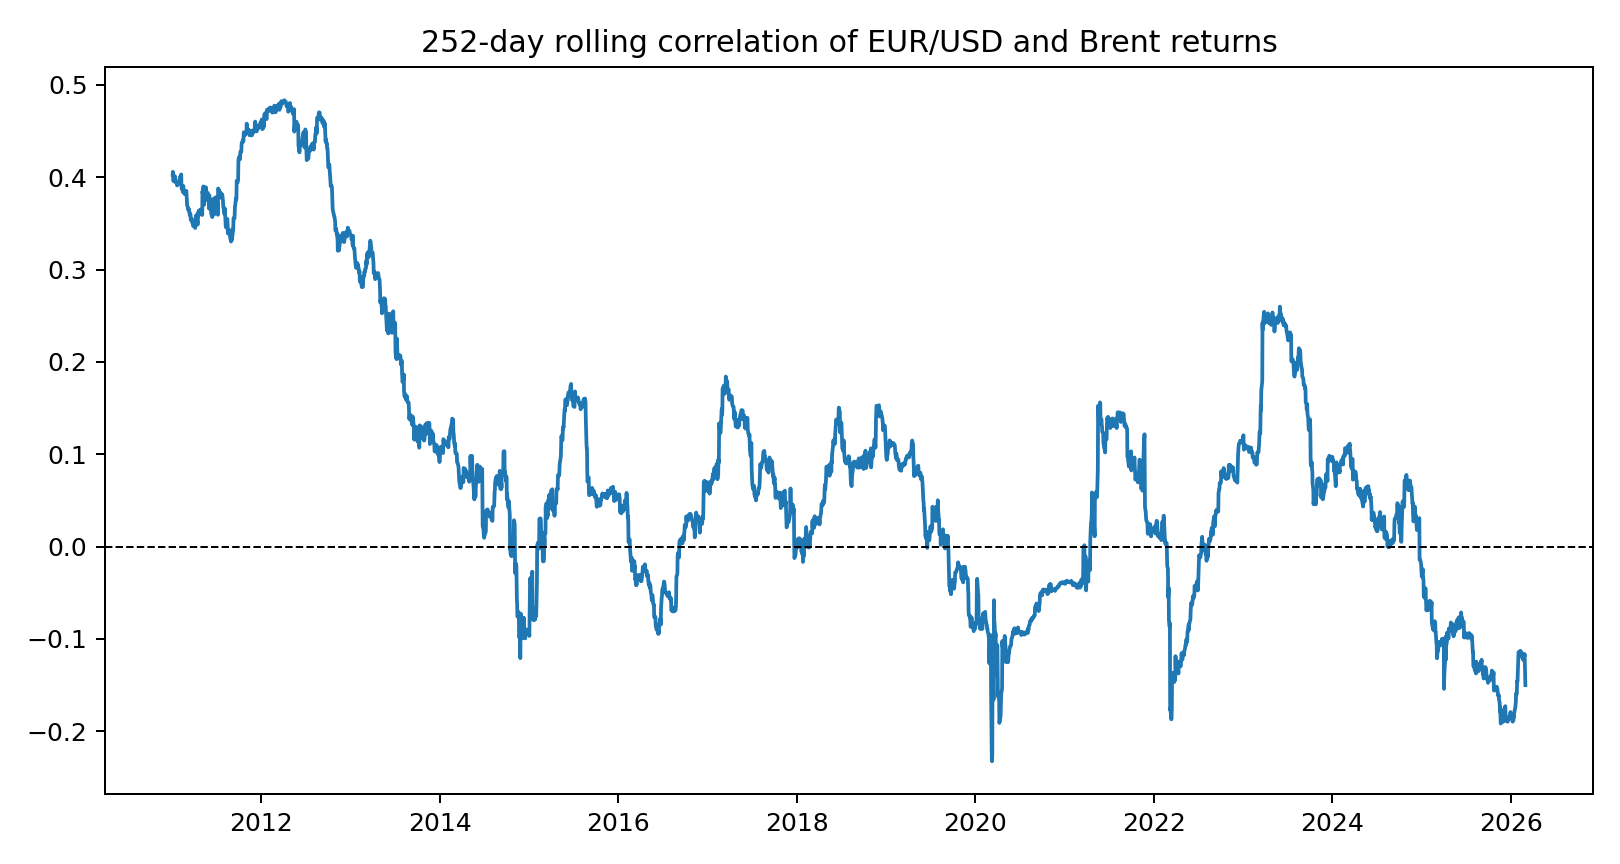
\includegraphics[width=0.88\textwidth]{results/rolling_correlation.png}
\caption{252-дневная скользящая корреляция доходностей EUR/USD и Brent}
\end{figure}

Корреляция заметно меняется по времени и периодически проходит через ноль. Это еще раз подтверждает, что для инвестиционных решений нельзя полагаться на ``вечную'' константную связь между нефтью и валютой.

Для полноты приведу и диаграмму рассеяния дневных доходностей.

\begin{figure}[H]
\centering
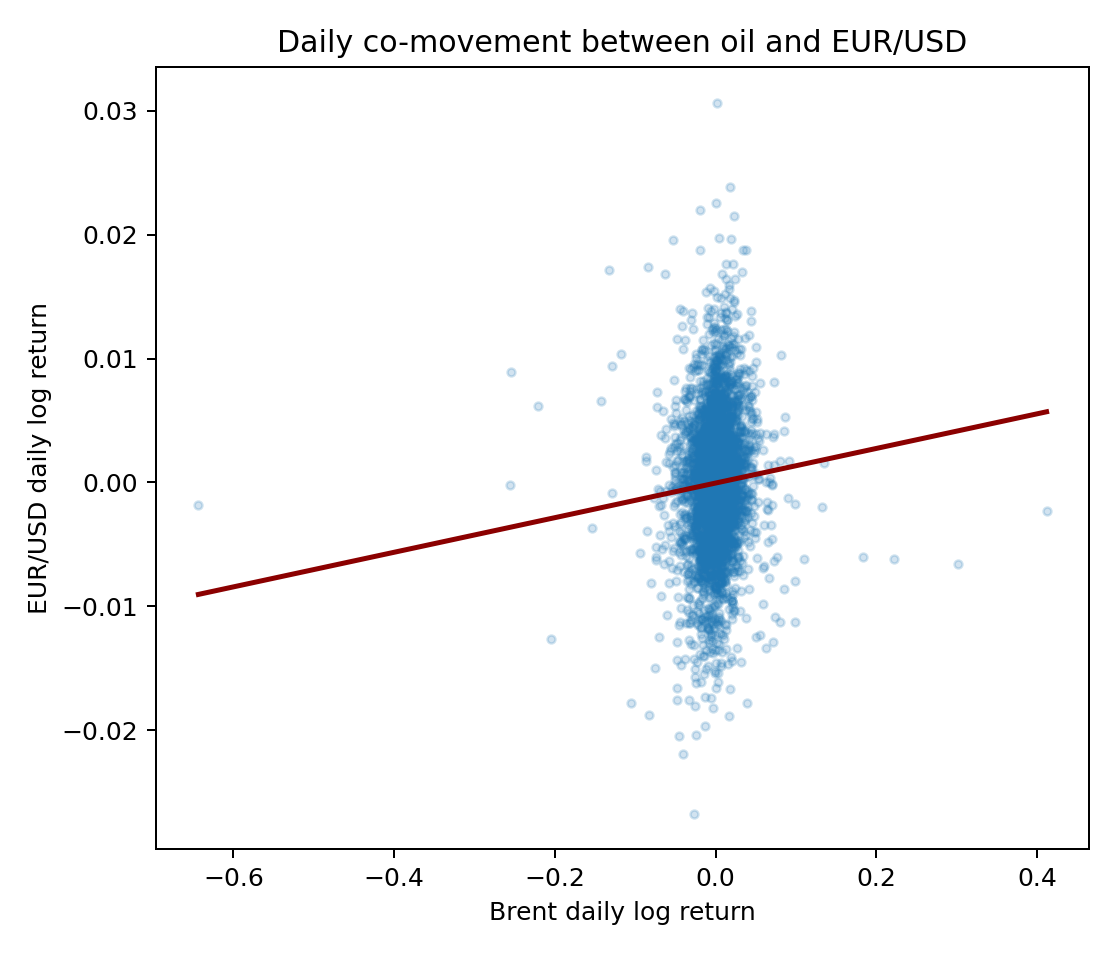
\includegraphics[width=0.68\textwidth]{results/scatter_daily.png}
\caption{Дневная совместная динамика доходностей Brent и EUR/USD}
\end{figure}

\textbf{Инвестиционная интерпретация.}
Если инвестор держит долларовый риск против евро, то рост нефти может быть полезным сигналом в кратком горизонте: исторически он сопровождался умеренным ростом EUR/USD. Но использовать одну только нефть как предиктор недостаточно, потому что после 2022 года объясняющая сила этого фактора заметно снизилась. Значит, для практической стратегии нефть разумно включать не как единственный сигнал, а как один из факторов в многомерной модели.

\section*{6. Отчет о проделанной работе}
За время выполнения проекта я сделал следующее.
\begin{enumerate}
    \item Изучил три статьи по теме и выписал из них основные гипотезы: наличие связи, возможную смену режимов и различие между долгосрочным и краткосрочным эффектом.
    \item Подобрал открытые данные, которые можно автоматически скачать и перепроверить.
    \item Написал воспроизводимый Python-скрипт для очистки данных, построения регрессий, тестов и графиков.
    \item Проверил стационарность и коинтеграцию, чтобы не смешивать уровни и доходности без эконометрического обоснования.
    \item Получил эмпирический результат: краткосрочная положительная связь между нефтью и EUR/USD есть, но она слабее после 2022 года; сильной устойчивой долгосрочной причинности данные не показывают.
    \item Подготовил отчет, таблицы, графики и отдельную презентацию для устного выступления.
\end{enumerate}

\section*{7. Вывод}
По результатам проекта можно сделать три главных вывода.

\begin{itemize}
    \item Между нефтью Brent и курсом EUR/USD действительно есть положительная краткосрочная связь: рост нефти в среднем сопровождается ростом EUR/USD, то есть относительным ослаблением доллара.
    \item Эта связь нестабильна по времени. До 2022 года она проявляется отчетливее, а в последние годы статистически почти исчезает.
    \item Для задач оптимального инвестирования нефть полезна как дополнительный фактор хеджирования и мониторинга валютного риска, но строить стратегию только на одном нефтяном индикаторе нельзя.
\end{itemize}

Итак, моя итоговая постановка подтверждается частично: \textit{нефть и EUR/USD связаны, но прежде всего в краткосрочной динамике и не во всех рыночных режимах одинаково сильно.}

\begin{thebibliography}{9}
\bibitem{benlaria2020}
Benlaria H., Gheraia Z., Belbali A. et al.
\textit{The Relationship between Crude Oil Prices, EUR/USD Exchange Rate and Gold Prices}.
International Journal of Energy Economics and Policy, 2020.

\bibitem{ecb2014}
Fratzscher M., Schneider D., Van Robays I.
\textit{Oil Prices, Exchange Rates and Asset Prices}.
ECB Working Paper No. 1689, July 2014.

\bibitem{dias2025}
Dias R., Galv\~ao R., Alexandre P. et al.
\textit{The Influence of the International Oil Price on the EUR/USD Exchange Rate}.
Journal of Ecohumanism, 2025.

\bibitem{fred}
Federal Reserve Bank of St. Louis.
\textit{FRED Data Series DEXUSEU and DCOILBRENTEU}.
\url{https://fred.stlouisfed.org/}
\end{thebibliography}

\end{document}
